\documentclass[border=10pt]{standalone}

\usepackage{tikz}
\usepackage{tikzsymbols}
\usetikzlibrary{calc,patterns,shapes.geometric}

\def\centerarc[#1](#2)(#3:#4:#5){\draw[#1] ($(#2)+({#5*cos(#3)},{#5*sin(#3)})$) arc (#3:#4:#5);}

\begin{document}
	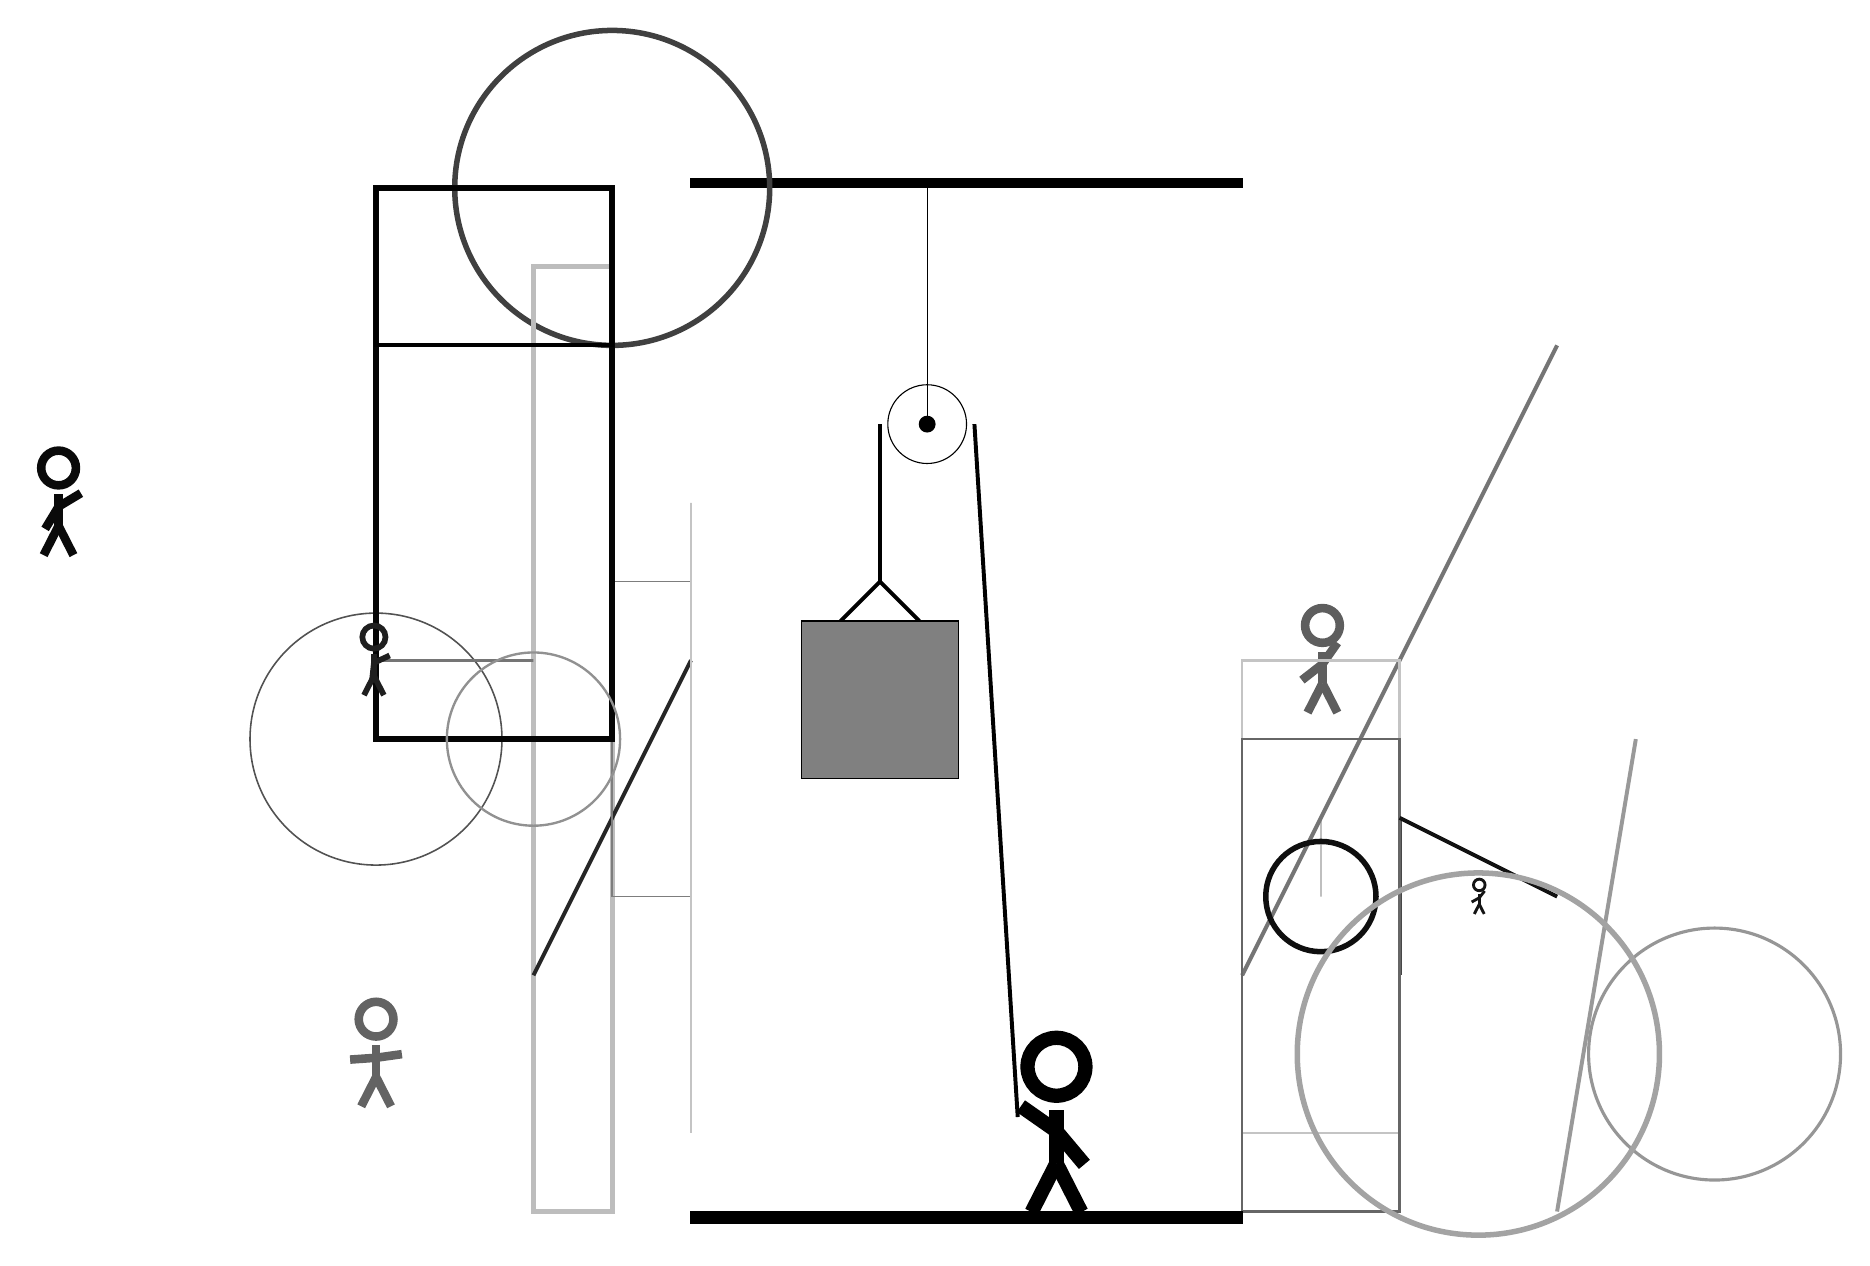
\begin{tikzpicture}
		%%%%% START %%%%%
		
		\draw[fill=black] (-2, 10) rectangle (5, 10.125);
		
		\draw (1, 7) circle (0.5);
		\draw[fill=black] (1, 7) circle (0.1);
		\draw (1, 10) -- (1, 7);
		
		\draw[line width=0.5mm] (-0.1, 4.5) -- (0.4, 5.0) -- (0.9, 4.5);
		\draw[fill=black!50] (-0.6, 4.5) rectangle (1.4, 2.5);
		
		\draw[line width=0.5mm] (0.4, 7) -- (0.4, 5.0);
		\centerarc[line width=0.5mm](1, 7)(0:180:0.6);
		\draw[line width=0.5mm](1.6, 7) -- (2.15, -1.8);
		
		\draw[line width=0.2mm, color=black!25] (6, 2) rectangle (6, 1);
		
		\draw[line width=0.5mm, color=black!72](7, 2) -- (7, 0);
		\draw[line width=0.5mm, color=black!54](5, 0) -- (9, 8);
		\draw [line width=0.7mm, color=black!75](-3, 10) circle (2.0);
		\node[line width=0.6mm, color=black!92] at (8, 1) {\Strichmaxerl[2][29][52]};
		\draw[line width=0.6mm, color=black!26] (-3, 9) rectangle (-4, -3);
		\draw[line width=0.5mm, color=black!85](-4, 0) -- (-2, 4);
		\draw [line width=0.2mm, color=black!68](-6, 3) circle (1.6);
		\node[line width=0.3mm, color=black!63] at (6, 4) {\Strichmaxerl[6][38][55]};
		
		\node[line width=0.6mm, color=black!96] at (-10, 6) {\Strichmaxerl[6][59][31]};
		\draw[line width=0.3mm, color=black!23] (7, -2) rectangle (5, 4);
		
		\draw[line width=0.2mm, color=black!51] (-2, 1) rectangle (-3, 5);
		\draw[line width=0.5mm, color=black!40](9, -3) -- (10, 3);
		
		\draw [line width=0.7mm, color=black!94](6, 1) circle (0.7);
		\draw[line width=0.4mm, color=black!54] (-4, 4) rectangle (-6, 4);
		\draw[line width=0.3mm, color=black!60] (5, -3) rectangle (7, 3);
		
		\draw[line width=0.3mm, color=black!23] (-2, -2) rectangle (-2, 6);
		\draw[line width=0.5mm, color=black!93](9, 1) -- (7, 2);
		\draw[line width=0.7mm, color=black!98] (-3, 3) rectangle (-6, 10);
		\node[line width=0.2mm, color=black!88] at (-6, 4) {\Strichmaxerl[4][84][25]};
		\draw[line width=0.5mm, color=black!100] (-3, 8) rectangle (-6, 10);
		
		\draw [line width=0.4mm, color=black!41](11, -1) circle (1.6);
		
		\draw [line width=0.7mm, color=black!36](8, -1) circle (2.3);
		\draw [line width=0.3mm, color=black!43](-4, 3) circle (1.1);
		\node[line width=0.5mm, color=black!61] at (-6, -1) {\Strichmaxerl[6][4][8]};
		
		
		\node at (2.6, -1.9) {\Strichmaxerl[10][-35][-50]};
		
		\draw[fill=black] (-2, -3) rectangle (5, -3.15);
		
		%%%%% END %%%%%
	\end{tikzpicture}
\end{document}